

%------------------------------------------------------------------------
\begin{frame}{مسئله شار بیشینه}
\begin{itemize}\itemr
\item
امّا چطور این کمیّت می‌تواند نماینده شار گذرنده از کل شبکه باشد؟
\item
برای درک بهتر این موضوع به شبکه شار به چشم یک بلوک بزرگ نگاه کنید که از رأس منبع شار به آن وارد و از مقصد خارج می‌شود.

\begin{figure}[h!]
\centering
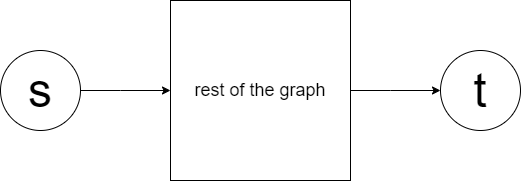
\includegraphics[width=.4\textwidth]{figs/chap01/6.png}
\end{figure}

\item
با توجه به قانون بقای شار، شار نمی‌تواند در این بلوک بزرگ بماند بنابراین با همان نرخی که وارد آن می‌شود باید از آن خارج شود. (فرض کنید پیکان‌ها شار خالص را نشان می‌دهند.)‌
\item
بنابراین نرخ خالص شار خروجی از منبع نماینده شاری است که در کل شبکه جریان دارد.
\end{itemize}
\end{frame}

%------------------------------------------------------------------------
\begin{frame}{مسئله شار بیشینه}
\framesubtitle{\quad فرض‌های ساده کننده}
\begin{itemize}\itemr
\item[-]
شاید دقت کرده باشید که در تعریف
در یک مسئله واقعی بیشینه‌سازی شار، ممکن است چند منبع تولید شار و چند مقصد داشته باشیم. در ادامه نشان می‌دهیم که چطور این مسئله به مسئله شار بیشینه عادی کاهش می‌یابد.

 مسئله شبکه شار با چندین رأس منبع و مقصد را می‌توان به یک شار با یک منبع و مقصد تبدیل کرد.

\item
\end{itemize}
\end{frame}
